\chapter{Physics at the LHC}\label{chap1}
\thispagestyle{empty}

In this chapter the Standard Model (SM) of particle physics is briefly described, in particular the main characteristics of the electroweak and strong interactions are discussed, as well as the mechanism of the electroweak symmetry breaking. Afterwards, few models that provide a simple extension of the SM Higgs sector are briefly described.
In addition, the phenomenology of Higgs boson production at LHC is described, focusing on its kinematic properties and, in particular, on the \hww decay channel. An overview of the main features of the Monte Carlo (MC) simulation techniques for the Higgs boson production are also given, as well as a brief report of the Higgs boson highlights from the experiments.

\noindent Unless otherwise stated, natural units $\hslash=c=1$ are used throughout this work.

\section{The Standard Model of particle physics}
%%%%%%%%%%%%%%%%%%%%%%%%%%%%%%%%%%%%%%%%%%%%%%%%%%%%%%%%%%%%%%%%%%%%%%
\label{sec:SM}

The Standard Model of Particle Physics (SM) is the theory that describes all fundamental constituents of matter and their interactions. It is a quantum field theory based on a $\mathrm{SU(3)_c \otimes SU(2)_L \otimes U(1)_Y}$ local gauge symmetry, and is capable to provide a quantitative description of three of the four interactions in nature: electromagnetism, weak interaction and strong nuclear force. During the past decades the predictions of the SM have been confirmed by experimental results with outstanding precision.

The SM can be divided in two sectors: the electroweak sector and the strong sector, known as Quantum Chromo-Dynamics (QCD). The aforementioned symmetry holds only if the fermion fields are massless, in contrast with the experimental observations of massive fermions. A mechanism, known as \emph{spontaneous symmetry breaking}, is introduced in the SM allowing the elementary particles to acquire mass. This mechanism requires the presence of a new field, known as Higgs field.

%\section{Electroweak interaction}
%%%%%%%%%%%%%%%%%%%%%%%%%%%%%%%%%%%%%%%%%%%%%%%%%%%%%%%%%%%%%%%%%%%%%%
\label{sec:EW}

The theory of electroweak interaction was formulated in the 1960s by S. L. Glashow, A. Salam and S. Weinberg~\cite{Glashow:1961tr,Weinberg:1967tq} as an $\mathrm{SU(2) \otimes U(1)}$ local gauge theory.
In 1957 the experiments lead by Madame Wu~\cite{Wu:1957my} and Garwin-Lederman-Weinrich~\cite{Garwin:1957hc} confirmed that the parity symmetry is maximally violated for weak charged current interactions, proving that only left-handed particles or right-handed antiparticles are involved in these interactions. 

To express this aspect the weak charged currents can be written making use of the Dirac spinors, $\ell$ and $\nu_\ell$ (representing the lepton and neutrino spinors, repsectively), as follows:

\begin{equation}
\begin{split}
J_\mu^+ &= \bar{\nu}_\ell \gamma_\mu \dfrac{1}{2}(1-\gamma^5) \ell \quad, \\
J_\mu^- &= \bar{\ell} \gamma_\mu \dfrac{1}{2}(1-\gamma^5)\nu_\ell \quad,
\end{split}
\end{equation}

where the ``$+$'' and ``$-$'' superscripts indicate the charge-raising and charge-lowering character of the currents, and $\gamma^5 = i\gamma^0\gamma^1\gamma^2\gamma^3$ is the product of the Dirac $\gamma$ matrices. In fact, the effect of the projector $P=\dfrac{1}{2}(1-\gamma^5)$ is to project the spinor to its left-handed component. Therefore, introducing the following doublet:

\begin{equation}
\chi_L = \begin{pmatrix} \nu_\ell \\ \ell \end{pmatrix}_L \quad ,
\end{equation}

where $L$ denotes the left-handed component of the spinor, and defining the ``step-up'' and ``step-down'' operators $\tau_\pm = \dfrac{1}{2}(\tau_1 \pm i\tau_2)$, where $\tau_i$ are the Puali matrices, the charged currents become:

\begin{equation}
\begin{split}
J_\mu^+ &= \bar{\chi}_L \gamma_\mu \tau_+ \chi_L \quad, \\
J_\mu^- &= \bar{\chi}_L \gamma_\mu \tau_- \chi_L \quad.
\end{split}
\end{equation}

In order to complete the $\mathrm{SU(2)}$ invariance of the theory, a third conserved current should exist with the form:

\begin{equation}
J_\mu^3 = bar{\chi}_L \gamma_\mu \dfrac{1}{2} \tau_3 \chi_L = \dfrac{1}{2}\bar{\nu}_L \gamma_\mu \nu_L -  \dfrac{1}{2}\bar{\ell}_L \gamma_\mu \ell_L \quad,
\end{equation}

The three currents $J_\mu^\pm$ and $J_\mu^3$ constitute an isospin triplet of weak currents. Nevertheless, $J_\mu^3$ cannot be identified with the weak neutral current, because the weak neutral current involves both left- and right-handed components. The electromagnetic current cannot be represented by $J_\mu^3$ as well, for the aforementioned reasons and because it cannot be coupled with the uncharged neutrino.

In order to save the $\mathrm{SU(2)}$ symmetry, the existence of a new $\mathrm{U(1)}$ symmetry is required, and a new conserved current arises.

%\section{The Higgs mechanism}
%%%%%%%%%%%%%%%%%%%%%%%%%%%%%%%%%%%%%%%%%%%%%%%%%%%%%%%%%%%%%%%%%%%%%%
\label{sec:Higgs}


%\section{The strong interaction}
%%%%%%%%%%%%%%%%%%%%%%%%%%%%%%%%%%%%%%%%%%%%%%%%%%%%%%%%%%%%%%%%%%%%%%
\label{sec:QCD}


\section{Beyond the Standard Model}
%%%%%%%%%%%%%%%%%%%%%%%%%%%%%%%%%%%%%%%%%%%%%%%%%%%%%%%%%%%%%%%%%%%%%%
\label{sec:BSM}

The discovery of the new boson in accordance with the Higgs boson predicted by the SM has been a major breakthrough in the contemporary particle physics. The Higgs boson mass is a free parameter in the SM and its measurement fixes all the other parameters related to the Higgs field, such as the coupling strengths with bosons and fermions. The current quest is to establish whether the properties of the discovered boson are consistent with the SM predictions, or it is only a component of a more entangled Higgs sector. Moreover, there are still several aspects that are not explained by the SM, such as the hierarchy problem or the nature of dark matter~\cite{Langacker:2010zza}.

Several theoretical models have been proposed to explain the deficiencies of the SM. One of the simplest extension of the SM Higgs sector requires the existence of an additional singlet scalar field, S, which is neutral under all quantum numbers of the SM gauge group~\cite{Robens:2015gla}. In general the singlet field mixes with the SM Higgs boson, H, allowing it to couple to the same states as the SM Higgs boson itself. If the mass of the scalar singlet was more than twice that of the SM Higgs boson, the S branching ratios would be reduced with respect to the H ones, because of the opening of the new $\mathrm{S \to HH}$ decay channel.

Identifying as H the observed Higgs boson with $m_\mathrm{H} = 125$\GeV, and supposing that the new scalar singlet S is heavier than H, one can introduce the scale factors of the low and high mass state couplings, $\mathcal{C}$ and $\mathcal{C'}$, respectively. These factors are bounded by the unitarity condition $\mathcal{C}^2 + \mathcal{C'}^2 = 1$. The singlet cross section and width are consequently modified by the factors $\mu'$ and $\Gamma'$, respectively:
\begin{equation}
\begin{split}
\mu' &= \mathcal{C'}^2 \cdot (1 - \mathcal{B}_\mathrm{new}) \quad ,\\
\Gamma' &= \Gamma_\mathrm{SM} \cdot \frac{\mathcal{C'}^2}{1 - \mathcal{B}_\mathrm{new}} \quad ,
\end{split}
\end{equation}

\noindent where $\mathcal{B}_\mathrm{new}$ is the singlet branching ratio to HH.

Other models, such as the \emph{two-Higgs-doublet model} (2HDM)~\cite{Branco:2011iw}, extend the minimal Higgs content requiring the introduction of a second Higgs doublet. 
The generalization of the SM Lagrangian with two complex scalar fields, which are $\mathrm{SU(2)_L}$ doublets, eventually gives rise to five physical Higgs bosons: a charged pair ($\mathrm{H^{\pm}}$); two neutral $CP$-even scalars (H and h, where $m_{\rm H}>m_{\rm h}$ by convention); and a neutral $CP$-odd scalar (A)~\cite{Craig:2013hca}. The parameter space of these 2HDM models can accommodate a wide range of variations in the production and decay modes of the SM-like Higgs boson. Nevertheless, tight constraints on flavour-changing neutral currents disfavour 2HDM with tree-level flavour violation. Similarly, limits on additional sources of $CP$ violation favour 2HDM with a $CP$-conserving potential. These assumptions significantly reduce the parameter space of 2HDM models. Moreover, if the h boson is identified with the observed 125\GeV boson, the experimental measurements further constrain the possible production and decay modes of the other predicted particles. Examples of possible decay channels in this framework are the following: the  heavy  $CP$-even  Higgs boson  may  decay  to  two  light  CP-even  Higgs bosons, $\mathrm{H \to hh}$; the $CP$-odd pseudoscalar Higgs boson may decay to a light $CP$-even Higgs and a Z boson, $\mathrm{A \to Zh}$; the charged Higgs bosons may decay to a SM-like Higgs and a $\mathrm{W}^\pm$ boson, $\mathrm{H^\pm \to \mathrm{W}^\pm h}$.

In order to search for new particles that could be ascribed to the simple models depicted above, or even to more complicated theories, it is of utmost importance to provide precise measurements of the Higgs boson couplings and kinematics, as well as its spin and parity properties. A complementary strategy is to perform direct searches for additional Higgs bosons in the full mass range accessible to current and future experiments.

\section{Phenomenology of proton proton interactions}
%%%%%%%%%%%%%%%%%%%%%%%%%%%%%%%%%%%%%%%%%%%%%%%%%%%%%%%%%%%%%%%%%%%%%%
\label{sec:ppInt}


\section{Higgs boson phenomenology}
%%%%%%%%%%%%%%%%%%%%%%%%%%%%%%%%%%%%%%%%%%%%%%%%%%%%%%%%%%%%%%%%%%%%%%
\label{sec:HiggsPheno}

In this section the Higgs boson production modes and decay channels are described, spending some time on the description of the \hww channel, which is the channel investigated in this work. Afterwards, a description of the effects due to higher order QCD corrections on Higgs boson kinematic variables is shown. Finally, a brief review of the Monte Carlo (MC) generators used for the simulation of Higgs boson processes is given.

%One of the main goals of the LHC was the search for the SM Higgs boson over a wide range of masses. This goal has been achieved in 2012, when the ATLAS and CMS collaborations announced the discovery of a new boson with mass $m_\mathrm{H} = 125$\GeV~\cite{Aad:2012tfa,Chatrchyan:2012xdj}, consistent with the SM Higgs boson prediction.




%%%%%%%%%%%%%%%%%%%%%%%%%%%%%%%%%%%%%%%%%%%%%%%%%%%%%%%%%%%%%%%%%%%%%%
\subsection{Higgs boson production mechanisms and decay channels}

The main processes contributing to the Higgs boson production at hadron colliders are represented by the Feynman diagrams shown in Fig.~\ref{fig:higgs_prod}.

\begin{figure}[htb]
\centering
\subfigure[ggH]{
 \includegraphics[width=0.45\textwidth]{images/ggH.pdf}
}
\subfigure[VBF]{
 \includegraphics[width=0.45\textwidth]{images/VBF.pdf}
}\\
\subfigure[VH]{
 \includegraphics[width=0.45\textwidth]{images/VH.pdf}
}
\subfigure[\ttH]{
 \includegraphics[width=0.45\textwidth]{images/ttH.pdf}
}
\caption{Main Higgs boson production processes at LHC.}\label{fig:higgs_prod}
\end{figure}

In order of decreasing cross section, the Higgs boson production modes are:

\begin{itemize}
\item \emph{Gluon fusion} (ggH): this is the main Higgs boson production mode at LHC over the whole mass spectrum. The process involves the fusion of two incoming gluons that give rise to the Higgs boson through a heavy quark loop, whose main contribution comes from the top quark, as shown in Fig.~\ref{fig:higgs_prod}(a).

\item \emph{Vector Boson Fusion} (VBF): each of the two interacting quarks emit a W or Z boson which, in turn, interact to produce the Higgs boson, as shown in Fig.~\ref{fig:higgs_prod}(b). Quarks deriving from the incoming partons after the emission of vector bosons proceed in the forward direction and represent the peculiar signature of this production mode, i.e. two high energy forward jets separated by a large pseudorapidity gap. This process has a cross section which is one order of magnitude lower than ggH for a large range of $m_\mathrm{H}$ values and it becomes comparable to ggH only for masses of the order of 1\TeV.

\item \emph{Vector boson associated production} (VH): also known as \emph{Higgsstrahlung}, this process is characterized by the emission of a Higgs boson from a $\mathrm{W}^\pm$ or Z boson produced by two incoming quarks, as depicted in Fig.~\ref{fig:higgs_prod}(c). The VH cross section is several orders of magnitude lower than the ggH and VBF cross sections.

\item \emph{Top quark associated production} (\ttH): a pair of top quarks, originated from the splitting of two incoming gluons, interacts to give rise to a Higgs boson, as illustrated in Fig.~\ref{fig:higgs_prod}(d).
\end{itemize}

\noindent Another production mechanism analogous to the \ttH process and with a similar cross section is the b quark associated production.

The SM Higgs boson production cross section for the various production modes depends on the Higgs boson mass and on the centre-of-mass energy, as shown in Fig.~\ref{fig:higgs_xsec}. In general, the production cross section of all processes decreases with increasing the Higgs boson mass, while the raise of the centre-of-mass energy reflects in an increase of the cross section over the whole mass range.

\begin{figure}[htb]
\centering
\subfigure{
 \includegraphics[width=0.45\textwidth]{images/XS_8TeV.pdf}
}
\subfigure{
 \includegraphics[width=0.45\textwidth]{images/totalXS.pdf}
}
\caption{Higgs boson cross section as a function of $m_\mathrm{H}$ for the various production mechanisms (left) and for different centre-of-mass energies (right).}\label{fig:higgs_xsec}
\end{figure}

The Higgs boson can decay to a variety of final states that can be divided in bosonic channels, like $\gamma\gamma$, ZZ or $\mathrm{W^+W^-}$, and fermionic channels, like $\tau\tau$, $\mathrm{b\bar b}$, etc.
Its branching ratio depends on the Higgs boson mass, as illustrated in Fig.~\ref{fig:higgs_br}, where different decay channels are compared over the whole mass spectrum. At $m_\mathrm{H} = 125$\GeV the decay channel with the largest branching ratio is $\mathrm{b\bar b}$, followed by WW, $\tau\tau$, ZZ and others. Although being the channel with the largest branching ratio, analyses looking at the H$\to \mathrm{b \bar b}$ decays are in practical cases limited by the overwhelming background contribution, which makes it possible only if the Higgs boson is produced via VBF, VH or \ttH, where additional jets or leptons can be used to tag the events.

The branching ratio to the WW and ZZ decay channels are instead dominant when increasing the Higgs boson mass, because the decays to real vector boson pairs become energetically allowed. In particular, the H$\to \mathrm{W^+W^-}$ decay channel, which is described in Sec.~\ref{sec:HWW}, is the second channel in terms of signal yield at $m_\mathrm{H} = 125$\GeV and the first one for higher mass values. Moreover, these channels are characterized by a much cleaner signature if the leptonic decays of one or both vector bosons are sought.

\begin{figure}[htb]
\centering
%\subfigure{
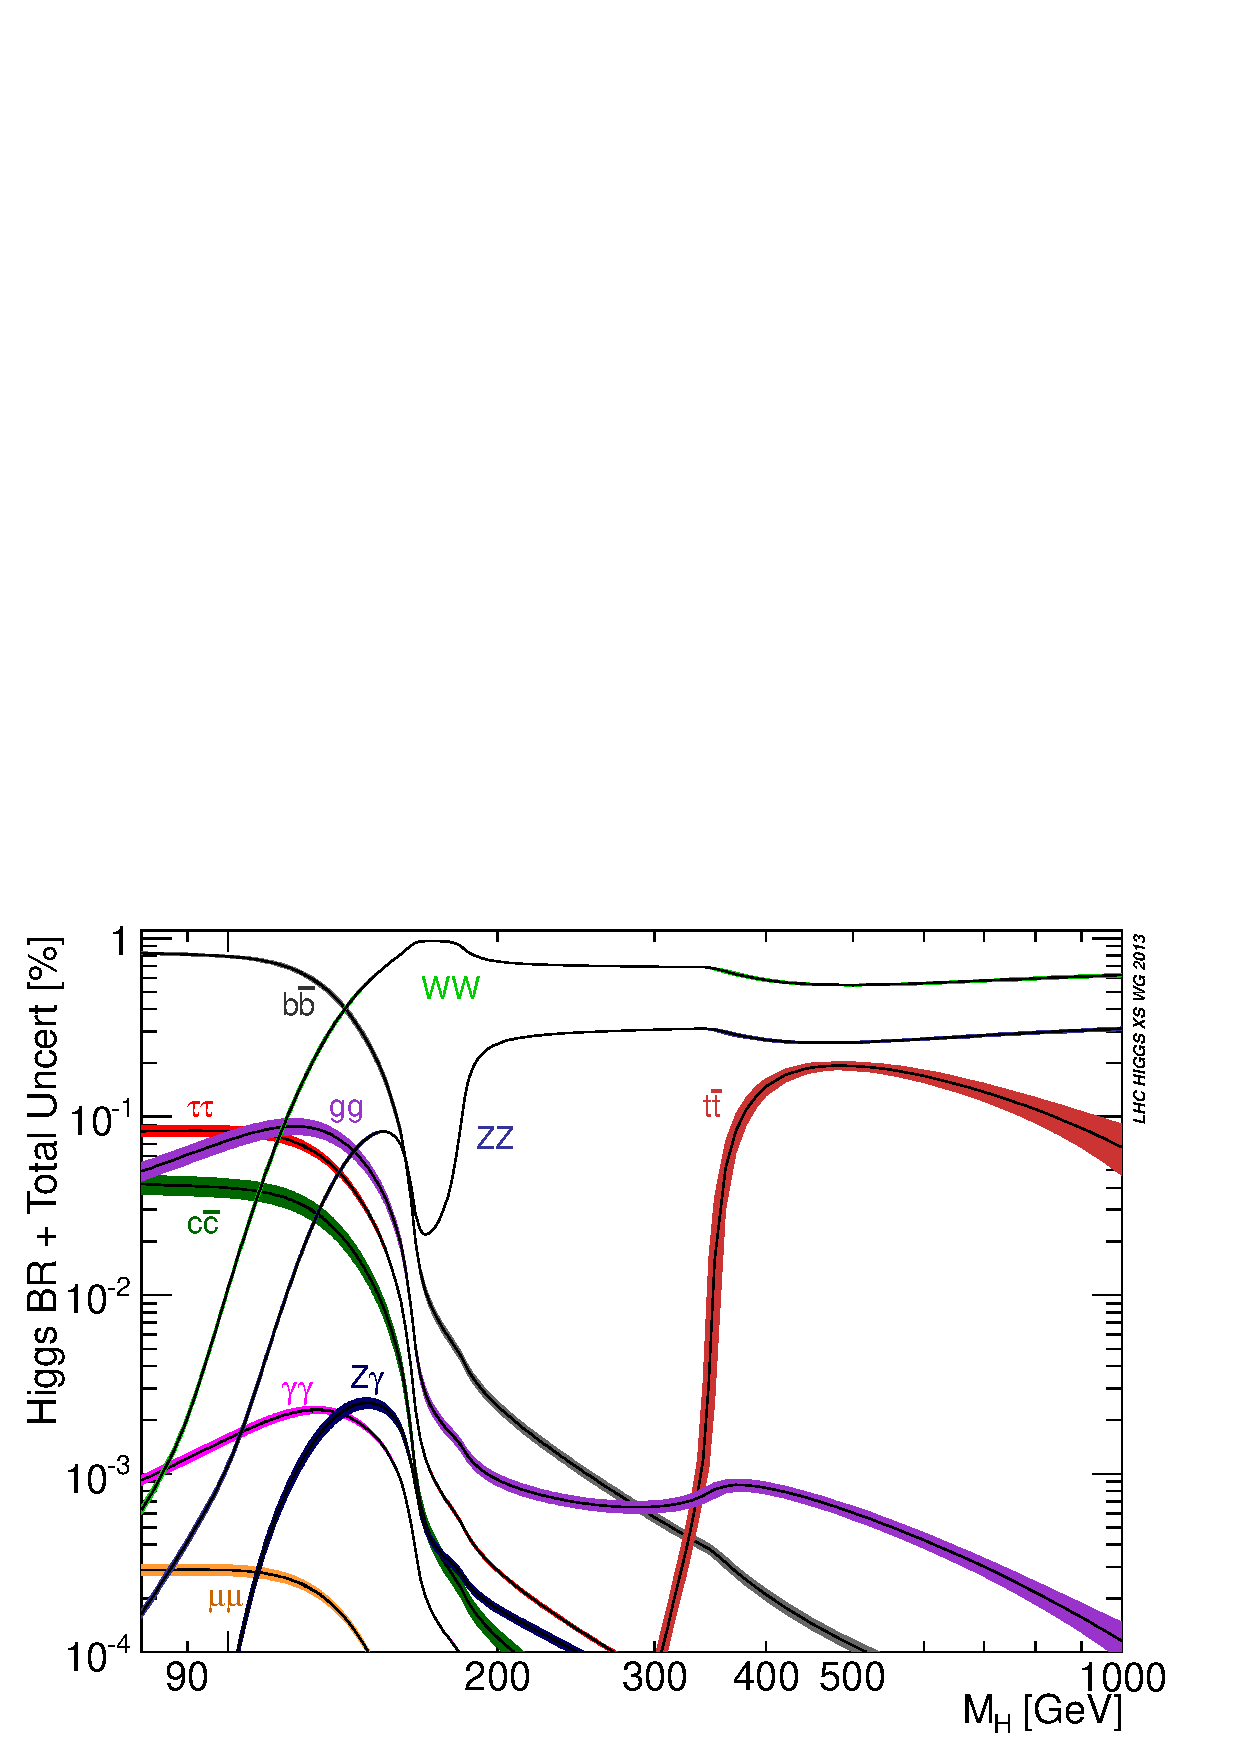
\includegraphics[width=0.6\textwidth]{images/Higgs_BR.pdf}
%}
%\subfigure{
% 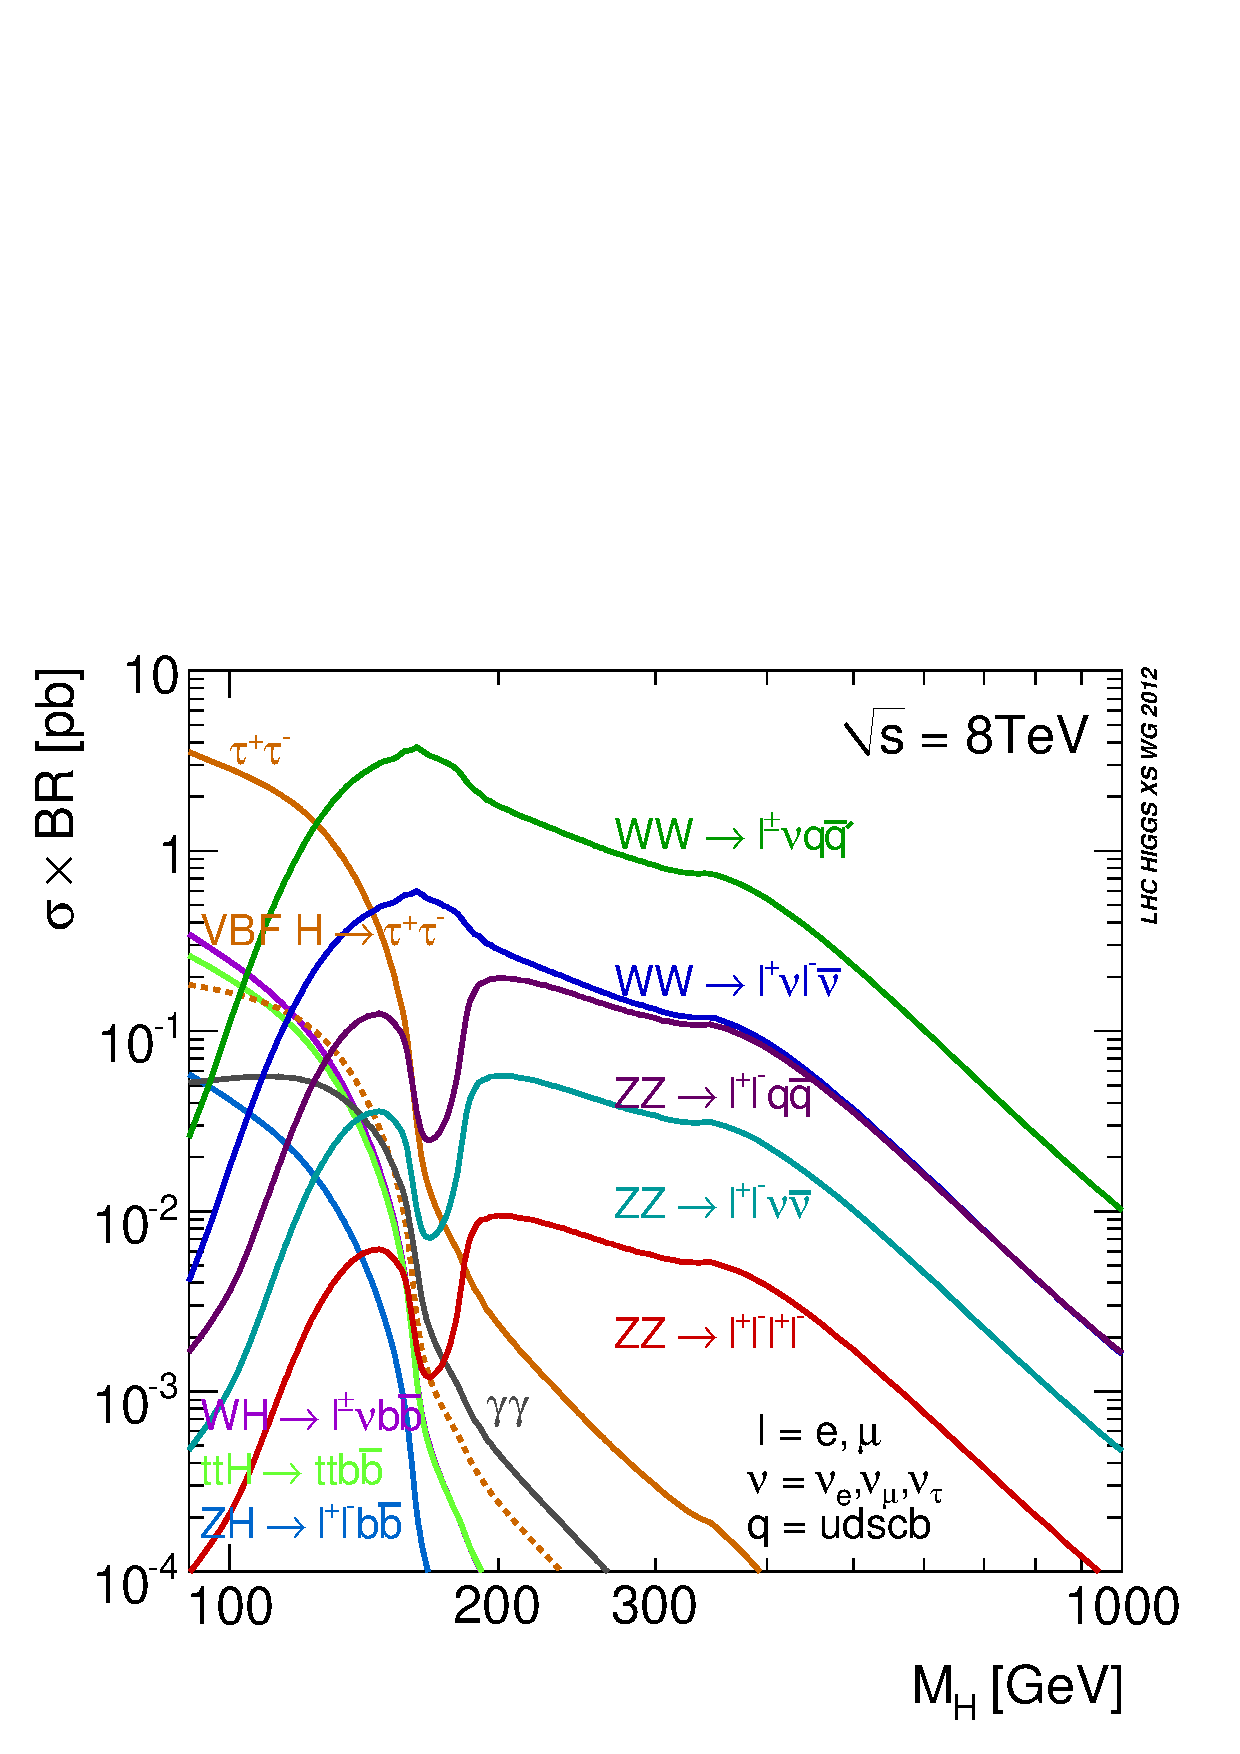
\includegraphics[width=0.45\textwidth]{images/Higgs_BR_2.pdf}
%}
\caption{Higgs boson branching ratio for all the decay channels as a function of $m_\mathrm{H}$.}\label{fig:higgs_br}
\end{figure}



%%%%%%%%%%%%%%%%%%%%%%%%%%%%%%%%%%%%%%%%%%%%%%%%%%%%%%%%%%%%%%%%%%%%%%
\subsection{The \hww decay channel}\label{sec:HWW}
As stated in the previous section, the \hww decay channel is one of the channels with the largest branching ratio across the full Higgs boson mass range. For Higgs boson masses below two times the W boson mass, $m_\mathrm{H} < 2m_\mathrm{W}$, the decay to two real W bosons is energetically forbidden, therefore one of the two is produced \emph{off-shell}. The W boson can in turn decay to hadrons, with a branching ratio of 67.41\%, or to leptons ($\mathrm{W}\to\ell\nu$) with a branching ratio of 10.86\%. The fully hadronic decay $\mathrm{H\to W^+W^- \to 4q}$ is thus the most probable decay mode, but the presence of four jets in the final state makes it hard to separate the signal from the overwhelming background contribution. The semi-leptonic final state, where one W boson decays to leptons and the other to hadrons, still has a large branching ratio and the presence of one electron or muon can be exploited to tag the events. Nevertheless the background contribution is, even in this case, very large.

The analyses presented in this work are focused on the fully leptonic final state (\hwwllnn) which, despite the lower branching ratio with respect to the other decay modes, is characterized by a clean signature and affected by much less background contribution. The signature of this final state is characterized by two leptons with opposite charge and a moderate amount of missing transverse energy, due to the presence of two neutrinos in the final state. In general the two leptons are characterized by high \pt values and, in case one of the W boson is off-shell (as for the SM Higgs boson case), the corresponding lepton has on average a smaller \pt with respect to the one arising from the on-shell W boson.

The final state with two same flavour leptons is not taken into account in the analyses discussed in this work, since it provides a smaller signal significance with respect to the different flavour case due to the presence of the huge contamination from Drell-Yan background processes.

Because of the presence of missing transverse energy in the final state, is not possible to reconstruct the full Higgs boson mass in this channel, and other methods must be used to distinguish between signal and background contributions.

The most important background processes contributing to this final state are non-resonant $\mathrm{q\bar q \to W^+W^-}$ and \ttbar production, whose Feynman diagrams are illustrated in Fig.~\ref{fig:wwandtop}. The first one is characterized by a final state identical to the signal, while the latter has two additional b quarks arising from the top quark decay. Despite the same final state, the lepton kinematics for signal and $\mathrm{q\bar q \to W^+W^-}$ processes is rather different. For the signal process, the W boson originates from a spin-0 particle decay and their spins must therefore be antiparallel, implying that the charged leptons produced in their decays appear preferentially in the same hemisphere~\cite{Ellis:2012wg}. In contrast, there is no preferential spin direction in the background case.
For this reason the azimuthal angle difference between the two leptons is on average smaller for signal than for background, resulting in a smaller dilepton invariant mass in the former case.

\begin{figure}[htb]
\centering
\subfigure[$\mathrm{q\bar q \to W^+W^-}$]{
  \includegraphics[width=0.4\textwidth]{images/WW.pdf}
}
\subfigure[\ttbar]{
  \includegraphics[width=0.4\textwidth]{images/ttbar.pdf}
}
\caption{Feynman diagrams corresponding to the $\mathrm{q\bar q \to W^+W^-}$ (left) and \ttbar (right) processes. The \ttbar diagram represents just one of the possible ways to produce a pair of top quarks at hadron colliders.}\label{fig:wwandtop}
\end{figure}

Other sub-dominant backgrounds arise from single top quark (tW, s-channel or t-channel), Drell-Yan, W+jets, di-boson and tri-boson processes.


%%%%%%%%%%%%%%%%%%%%%%%%%%%%%%%%%%%%%%%%%%%%%%%%%%%%%%%%%%%%%%%%%%%%%%
\subsection{Higgs boson kinematics}

The Higgs boson production at hadron colliders is kinematically characterized by its transverse momentum, \pth, and pseudorapidity, $\eta$. The $\eta$ distribution is essentially driven by the PDF of the partons in the colliding hadrons and it is only mildly sensitive to radiative corrections. The \pth distribution is instead sensitive to QCD radiative corrections. 
Considering the ggH production mode, at LO in perturbation theory, $\mathcal{O}(\alpha_s^2)$, the Higgs boson is always produced with \pth equal to zero. Indeed in order to have \pt different from zero, the Higgs boson has to recoil at least against one parton. Higher order corrections to the ggH process are numerically large and are known at NLO including full top quark mass dependence~\cite{Spira:1995rr,Harlander:2005rq}, and at NNLO using the so-called large-$m_\mathrm{t}$ approximation~\cite{Ravindran:2003um,Catani:2007vq,Anastasiou:2015ema}, in which the top quark mass is assumed to be very large and the fermionic loop is replaced by an effective vertex of interaction. Starting from the NLO, the Higgs boson can be produced recoiling against other final state partons, resulting in finite \pth values. For this reason the LO process for Higgs production at $\pt \neq 0$ is at $\mathcal{O}(\alpha_s^3)$, and the counting of perturbative orders differs between inclusive Higgs boson production and \pth distribution. Also, NNLO QCD corrections in the \pth observable have recently been shown~\cite{Chen:2016zka}.

When $\pth \sim m_\mathrm{H}$ the QCD radiative corrections to \pth differential cross section are theoretically evaluated using fixed-order calculations. When $\pth \ll m_\mathrm{H}$ the perturbative expansion does not converge due to the presence of large logarithmic terms of the form $\alpha_s^n \ln^{2n}m_\mathrm{H}^2/\pt^2$, leading to a divergence of $d\sigma/d\pt$ in the limit of $\pt\to0$. For computing the \pth spectrum in this region, soft-gluon resummation techniques are used~\cite{Bozzi:2005wk,deFlorian:2012mx}, and matched to the fixed-order calculation in the $\pth \sim m_\mathrm{H}$ region.
For the \pth differential cross section the large-$m_\mathrm{t}$ calculation is a crude approximation, since it is known that the top quark mass has a non-negligible effect on the shape of the spectrum. Moreover the inclusion of the bottom quark contribution in the fermionic loop can significantly modify the \pth shape~\cite{Grazzini:2013mca}, as shown in Fig.~\ref{fig:pth_quarkmass}. Hence, a precise experimental measurement of the \pth spectrum is important to test the existing SM calculations. 

\begin{figure}[htb]
\centering
\includegraphics[width=0.5\textwidth]{images/pth_quarkmass.png}
\caption{Distribution of \pth computed at NLO ($\alpha_s^4$) and divided by the calculation obtained in the large-$m_\mathrm{t}$ approximation. The red dashed line corresponds to the calculation including the top quark mass while the blue line refers to the calculation including also the bottom quark effects.}\label{fig:pth_quarkmass}
\end{figure}

Possible extensions of the SM predict a modification of the Higgs boson couplings to gluons and top quarks. Many of these models actually predict the existence of new states that interact with the SM Higgs boson but are beyond the direct production reach at the actual LHC energies. The effect of these new states could however show up as a deviation of the Higgs boson couplings with respect to the SM expectation. The modification of the couplings, as shown in Refs.~\cite{Azatov:2013xha,Harlander:2013oja}, can change the kinematics of the Higgs boson production and the effect can be particularly sizeable in the tail of the \pth distribution. 
Other models, such as Composite Higgs~\cite{Marzocca:2012zn}, predict the existence of top-partners, which are heavy resonances with the same quantum numbers as the top quark, that can interact with the Higgs boson in the ggH fermionic loop, changing the \pth shape with respect to what the SM predicts~\cite{Banfi:2013yoa}.
The measurement of the \pth spectrum is thus a useful tool for indirect searches of new particles predicted by theories beyond the SM.





%%%%%%%%%%%%%%%%%%%%%%%%%%%%%%%%%%%%%%%%%%%%%%%%%%%%%%%%%%%%%%%%%%%%%%
\subsection{Event generators for Higgs boson production}

The structure of events produced at high energy colliders is extremely complex, and complex numeric simulations are necessary to effectively simulate realistic events. Monte Carlo (MC) event generators are programs that subdivide the problem of producing realistic events into a sequence of tasks that can be handled separately with the help of both analytic and numeric computations.

The production of hadron-hadron collision events is the result of the following chain of calculations:

\begin{itemize}
\item the first step consists in the calculation of cross section for the selected process, considering partons extracted from the incoming hadrons as free particles;

\item the event production starts with two colliding hadrons with given momenta. One parton out of each hadron is selected to enter the scattering process of interest. This step is often referred to as \emph{hard scattering} generation. Final state partons and leptons are produced according to the calculated differential cross sections;

\item resonances produced in the hard event are decayed;

\item when two partons take part in the hard event, accelerated colour charges are present, thus bremsstrahlung can occur. This effect is called initial state radiation (ISR) and is simulated with the so called \emph{Initial State Parton Showers} algorithm, using the knowledge of the PDFs;

\item also the final state partons can produce further radiation, called final state radiation (FSR), which is simulated by the \emph{Final State Parton Showers} algorithms;

\item in addition to the partons taking part in the hard interaction, several other parton pairs can interact during a hadron-hadron collision, giving rise to interactions with smaller transferred momentum. These \emph{multiple parton interactions} (MPI) contribute to the so called \emph{underlying event} (UE). Such interactions need to be well simulated to produce realistic events;

\item leftovers of the interacting hadrons need to be simulated to balance the colour charge
and four-momentum conservation. The beam remnant handling is thus another step in the event generation;

\item the partons produced in the final state after the hard scattering are not observed as free particles but are subjected to the hadronization process, that cannot be described with perturbative QCD and is simulated using empirical models;

\item finally, the event generator takes care of decaying $\tau$ leptons and B hadrons. Particles with very short lifetime are generally decayed by the generator itself, while those with longer lifetimes are left undecayed.
\end{itemize}

The calculation of the hard process cross section is performed using the Matrix Element (ME) method, which is available for a variety of processes and consists on the exact matrix element calculation of the Feynman diagram of the process of interest. This approach is performed using perturbative QCD calculations and provide an analytically exact solution. Tree-level cross sections can be calculated including up to several partons in the final state. Loop calculations are instead more complex and are available only for a limited set of processes. 

The ME method presents two complications: the first one arises from the presence in the calculation of partons with low transverse momentum (\emph{soft} divergence) and the second to situations in which the emitted parton is collinear to the radiating parton (\emph{collinear} divergence). Both these cases lead to divergences that spoil the perturbative calculation. The virtual corrections would cancel these divergences but, since at tree-level they are not included, the phase space has to be carefully tailored to avoid the problematic regions. This means that the matrix
element cross section calculations are performed away from soft and collinear divergences. Therefore, in order to produce realistic events, the phase space regions omitted in the ME calculation need to handled using a different method, the Parton Shower calculation.

Parton Shower (PS) algorithms offer an alternative way both to handle the complexity of several successive branchings and to remove soft and collinear divergences. The parton showers are described by the algorithm as a sequence of elementary events $a\to bc$, where each event can happen with a certain probability driven by the structure of perturbative QCD. The introduction of a threshold value
and the application of an angular sorting procedure in the emission of partons allows to eliminate soft and collinear divergences typical of the ME method. The parton cascade is evolved down to a certain virtuality, of the order of 1\GeV. After that, non perturbative effects take place and the hadronization is applied. Since the parton shower machinery relies on a collinear approximation of the matrix element, it is supposed to perform well in the description of the evolution of jets, but not to provide a precise description of configurations with well separated partons.

The two aforementioned techniques are therefore complementary and their combined application in the intermediate cases allows to exploit the characteristics of the two algorithms in the respective limits of validity. Several prescriptions exist to combine together the ME and PS calculations avoiding double-counting or holes in the phase space~\cite{Hoche:2006ph}.

In this work the \textsc{Powheg}~\cite{Kramer:2005hw,Frixione:2007vw,Lavesson:2008ah,Alioli:2008tz, Nason:2009ai} and \textsc{MadGraph} (and its evolution \textsc{MadGraph5\_aMC@NLO}) generators~\cite{Alwall:2014hca} are mostly used for the ME calculation, interfaced to \textsc{Pythia}~\cite{Sjostrand:2006za,Sjostrand:2007gs} for the PS and hadronization. 

\textsc{Powheg} is a ME event generator that performs calculations with NLO QCD accuracy and provides an easy prescription for the interface to PS programs. It can be used to generate events corresponding to a large number of predefined processes. It is used for the simulation of the majority of the processes involving Higgs boson production, as ggH and VBF. The \textsc{JHUGen}~\cite{JHUGen} generator, which is capable to take into account all spin correlations, is usually employed together with \textsc{Powheg} to simulate the Higgs boson decay to whatever final state is desired. In the analyses described in Chapter~\ref{chap4} two versions of this generator are used for simulating events produced via the ggH mechanism: \textsc{Powheg V1} and the more recent \textsc{Powheg V2}, which takes into account the finite mass of the bottom and top quarks in the ggH loop.

\textsc{MadGraph5\_aMC@NLO} is a software that allows to generate amplitudes and events for any user defined process (with up to 9 external particles) with LO or NLO QCD accuracy.

\textsc{Pythia} is a general purpose generator. It contains a large subprocess library covering SM and BSM physics. It can be used standalone as a ME generator to perform cross section calculation and generate events at LO QCD accuracy, or interfaced to a ME generator like \textsc{Powheg} or \textsc{MadGraph5\_aMC@NLO} as a PS and for the simulation of the hadronization process.


\section{Experimental Higgs boson highlights}
%%%%%%%%%%%%%%%%%%%%%%%%%%%%%%%%%%%%%%%%%%%%%%%%%%%%%%%%%%%%%%%%%%%%%%
\label{sec:HiggsExp}

The discovery of the new boson has been followed by a comprehensive set of measurements aimed at establishing the properties of the particle. Latest results reported by both the ATLAS and CMS experiments are consistent with the SM expectations for the Higgs boson. The properties that have been measured are, mainly:

\begin{itemize}
\item the signal strength modifier $\mu = \sigma/\sigma_\mathrm{SM}$, where $\sigma$ is the observed production cross section and $\sigma_\mathrm{SM}$ is the value predicted by the SM for a given mass hypothesis;

\item the couplings to bosons and fermions;

\item the spin and parity;

\item the total decay width of the resonance.
\end{itemize}

Moreover, the combination of the results of the two experiments has recently been performed concerning the mass of the new boson, which is found to be $m_\mathrm{H} = 125.09 \pm 0.21 ~\text{(stat.)} \pm 0.11~\text{(syst.)}$\GeV~\cite{Aad:2015zhl}.

The CMS experiment has investigated the Higgs boson decays to ZZ, WW, $\gamma\gamma$, $\tau\tau$ and $\mathrm{b \bar b}$ using 2011 and 2012 data, and is now looking at the same channels using new data collected at a centre-of-mass energy of 13\TeV. The 8\TeV CMS results of all the channels have been combined and the best-fit signal strength corresponding to the measured mass is found to be $\mu = 1.00 \pm 0.09~\text{(stat.)} ^{+0.08}_{-0.07}~\text{(theo.)} \pm  0.07~\text{(syst.)}$~\cite{Khachatryan:2014jba}, in good agreement with the SM expectation $\mu=1$.
The signal strengths modifiers obtained in different sub-combinations of channels for $m_\mathrm{H}=125$\GeV are shown in Fig.~\ref{fig:signal_strengths}, grouped by production mode tag and decay channel.

\begin{figure}[htb]
\centering
\includegraphics[width=0.7\textwidth]{images/signal_strengths.pdf}
\caption{Values of the best-fit $\mu$ for the overall combined analysis (solid vertical line) and separate combinations grouped by production mode tag and decay channel.}\label{fig:signal_strengths}
\end{figure}
    
The combination of all measurements in all decay channels is used to extract ratios between the observed coupling strengths and those predicted by the SM. The formalism used to test for deviations from the SM expectations has been established by the LHC Higgs Cross Section Working Group in Ref.~\cite{Heinemeyer:2013tqa}. This formalism makes some assumptions, in particular that the observed state has $J^P =0^+$ and that the narrow width approximation holds, leading to a factorization of the coupling strengths for production and decay modes. As an example, Higgs boson events produced via ggH and decaying to WW, i.e. $\mathrm{gg\to H\to WW}$, can be used to measure the Higgs boson coupling to W bosons and to fermions (mainly top quarks due to their presence in the gluon fusion loop). The combination of ATLAS and CMS results using data collected at 7 and 8\TeV is used to test the Higgs boson coupling to fermions $k_F$ and bosons $k_V$~\cite{Khachatryan:2016vau}. The contours at 68\% CL in the $(k_F^f, k_V^f)$ plane (where the $f$ refers to the generic decay channel H$\to f$) for the combination of ATLAS and CMS results and for the individual channels are shown in Fig.~\ref{fig:couplings}.

\begin{figure}[htb]
\centering
\includegraphics[width=0.7\textwidth]{images/couplings.pdf}
\caption{Contours at 68\% CL in the $(k_F^f, k_V^f)$ plane for the combination of ATLAS and CMS results and for the individual channels.}\label{fig:couplings}
\end{figure}

The combined result is in agreement with the SM expectation and the final confidence interval is driven by the \hww channel, which provides the most precise determination of $k_F^f$ and $k_V^f$ because it is the only channel that provides significant constraints on both parameters through the measurements of the ggH and VBF production processes.

About the spin and parity properties, the results of the H$\to \gamma\gamma$, H$\to$ZZ$\to 4\ell$ and \hwwllnn channels confirmed the hypothesis of a scalar boson ($J^P = 0^+$), excluding the other hypotheses with a confidence level of 99\% or higher.

The Higgs boson total decay width ($\Gamma_\mathrm{H}$) is predicted by the SM as a function of its mass, as shown in Fig.~\ref{fig:width}. At $m_\mathrm{H}=125$\GeV the Higgs boson is predicted to be a narrow resonance, with a total decay width of the order of 4.1\MeV. Direct measurements of the decay width have been performed in the H$\to$ZZ$\to 4\ell$ and H$\to\gamma\gamma$ channels, but the results are limited by the experimental resolution, which is about three orders of magnitude larger than the expected value, thus not allowing to provide significant constraints. The sizeable off-shell production of the Higgs boson can also be used to constrain its natural width. In fact, a measurement of the relative off-shell and on-shell production provides direct information on $\Gamma_\mathrm{H}$~\cite{Caola:2013yja}, under the assumption that the Higgs boson off- and on-shell production mechanisms are the same as in the SM and the ratio of couplings governing the two remains unchanged with respect to the SM predictions. Using this technique and combining the CMS results of the H$\to$ZZ$\to 4\ell$ and \hwwllnn channels, the upper limit at 95\% CL on the Higgs boson total decay width is found to be $\Gamma_\mathrm{H}^\mathrm{obs} < 13$\MeV~\cite{Khachatryan:2016ctc}, which represents a far better constraint with respect to direct measurements.

\begin{figure}[htb]
\centering
\includegraphics[width=0.7\textwidth]{images/width.pdf}
\caption{Total decay width of the SM Higgs boson as a function of $m_\mathrm{H}$.}\label{fig:width}
\end{figure}

Differential cross section measurements have also been performed by both experiments in the bosonic channels, $\gamma\gamma$, ZZ and $\mathrm{W^+W^-}$ (the latter is presented in Chapter~\ref{chap4} of this work), showing agreement with the SM-based theoretical predictions.

